\documentclass[10pt,twocolumn,letterpaper]{article}

\usepackage{cvpr}
\usepackage{times}
\usepackage{epsfig}
\usepackage{graphicx}
\usepackage{amsmath}
\usepackage{amssymb}
\usepackage{multirow}
\usepackage{booktabs}

% Include other packages here, before hyperref.

% If you comment hyperref and then uncomment it, you should delete
% egpaper.aux before re-running latex.  (Or just hit 'q' on the first latex
% run, let it finish, and you should be clear).
\usepackage[breaklinks=true,bookmarks=false]{hyperref}

\cvprfinalcopy % *** Uncomment this line for the final submission

\def\cvprPaperID{****} % *** Enter the CVPR Paper ID here
\def\httilde{\mbox{\tt\raisebox{-.5ex}{\symbol{126}}}}

% Pages are numbered in submission mode, and unnumbered in camera-ready
%\ifcvprfinal\pagestyle{empty}\fi
\setcounter{page}{1}
\begin{document}

%%%%%%%%% TITLE
\title{Evaluation of SD Filter for Multi-Spectral Image De-Noising}

\author{Mert Can Ergun\\
Hacettepe University\\
Department of Computer Engineering\\
{\tt\small mcergun@windowslive.com}
% For a paper whose authors are all at the same institution,
% omit the following lines up until the closing ``}''.
% Additional authors and addresses can be added with ``\and'',
% just like the second author.
% To save space, use either the email address or home page, not both
\and
Gokhan Yaliniz\\
Hacettepe University\\
Department of Computer Engineering\\
{\tt\small gokhanyaliniz@gmail.com}
}

\maketitle
%\thispagestyle{empty}

%%%%%%%%% ABSTRACT
\begin{abstract}
   Traditional de-noising algorithms using static and dynamic guidance images are already used. The SD Filter leverages both static and dynamic guidance together for many applications. For this project de-noising application is studied. The method uses high detail NIR image as a static guidance for de-noising an visible spectrum RGB image\cite{ham2015robust} In this project some other types of guided de-noising applications involving NIR, LWIR and Day-light imagery.
   
   To evaluate this method's performance some image metric methods are also studied in this paper. Their performance is evaluated on AWGN.
   
   Project is developed on github.com and code is available at \href{https://github.com/mcergun/CMP717-Project}{https://github.com/mcergun/CMP717-Project}
\end{abstract}

%%%%%%%%% BODY TEXT
\section{Introduction}

Many tasks in image processing requires regularization in order to get good results. Guidance is used to transfer strong structures from one image to another. 

Traditional methods use static or dynamic guidance images. Static guidance regularization modulates input image with similarities between two images. It can easily reflect internal properties of the input image.
Dynamic guidance regularization on the other hand modulates input image with similarities between neighboring pixels. It can preserve local features better than static guidance regularization.

Robust Image Filtering using Joint Static and Dynamic Guidance\cite{ham2015robust} paper uses both static and dynamic guidance images together to keep local features and static image structures intact.

Infrared sensors are still developing and thus there are some intrinsic problems with Infrared Imaging(IR). These problems will be dealt with during the project.

TRICLOBS(TRI-band Color Low-light OBServation) Dataset\cite{triclobs} is used for de-noising with multiple spectrum images of the same scene. The dataset includes different civilian or military scenarios executed against a special kind of hardware that records visible, NIR and LWIR spectrum. This database will be used in evaluation part of the method\cite{ham2015robust}.

%-------------------------------------------------------------------------
\section{Related Work}

Both static and dynamic guidance have their own advantages and disadvantages. To get better result B.Ham et al.\cite{ham2015robust} proposed a novel approach provides a unified model as using both static and dynamic guidance together for many applications, to handle most of the artifacts, and outperforms the state of the art in all the cases that can be seen using either static guidance and dynamic guidance.

To get a better understanding, we have investigated the static and dynamic guidance seperately through Robust Image Filtering using Joint Static and Dynamic
Guidance\cite{ham2015robust} . Static and dynamic guidance can be explicit or implicit. Implicit regularization stems from a filtering framework.\cite{ham2015robust}. 

The structure of the guidance image is transferred to input image by filtering using a weight function that depends on the similarity of features in the input images \cite{Kopf:2007:JBU:1275808.1276497}. The bilateral filter (BF)\cite{tomasi1998bilateral}, guided filter (GF) \cite{he2013guided}, and weighted median filter (WMF) \cite{ma2013constant} have been adapted to static guidance regularization successfully. There are two representative filtering methods dynamic
guidance are iterative nonlocal means (INM)  \cite{brox2008efficient} and the rolling-guidance filter (RGF) \cite{ham2015robust}. The filtering framework of this two approaches are the same but INM preserve texture during noise reduction, while The RGF removes texture through scale spae filtering. Even if the implementation of this implicit regularization is easy and simple, it suffers  when information is sparse, e.g., in image colarization \cite{levin2004colorization} or because of its local nature this approach might introduce artifacts, e.g., halos and gradient reversal  \cite{he2013guided}.The conditions  of implicity regularization is highly controlled, so it employed as a pre-processing and/or post-processing for further applications \cite{lang2012practical,ma2013constant}. Explicity encoding the regularization process into an objective functional is an alternative approach. Consistency between input and output images described by a fidelity term. A regularization term encourages to the ouput images to get same similar strcture between input and guidance images. These are two parts of the objective functionality.Existing regularization methods can be applied to limited range of application and have various artifacts. One of the most popular explicit regularization method that has been used  in static guidance regularization \cite{park2011high} is the weighted least-squares (WLS) framework \cite{farbman2008edge}. Anisotropic diffusion (AD) \cite{perona1990scale} is an explicit regularization framework using dynamic guidance. Quite the contrary INM \cite{brox2008efficient} and the RGF \cite{ham2015robust}, AD updates bot input and guidance images at every step iteratively. This regularization has more flexibility than implicit ones. It overcomes several limitations of implicit regularization such as halos and gradient reversal, at the cost of global intensity shifting \cite{farbman2008edge,he2013guided}.
B. Ham et al. propose a novel approach to unify both static and dynamic guidance to get both of their advantages. They applied their models to RGB/NIR and flash/non-flash denoising problems. It can be seen easily from their results, their methods handles most of the artifacts and outperforms the state of the art.Although their proposed model may look similar to WLS \cite{farbman2008edge} and the RGF \cite{yan2013cross}, their nonconvex objective function needs a different solver. Contrary to iteratively reweighted least-squares (IRLS) \cite{daubechies2010iteratively} regularizer but approximate the objective function by a surrogate (upper-bound) function.


\section{Methodology}
The project can be divided into two main parts. The methodology for each part will be discussed in following sections.

\subsection{Sigma Estimation}
IR imaging sensors are more complicated than visible light RGB sensors. One of the problems of IR sensors is higher amounts of noise. 

For most image processing applications, especially for image de-noising, there needs to be a way to measure image quality and enhancements between pre-algorithm and post-algorithm steps.

A widely used image quality metric is peak signal to noise ratio(PSNR). PSNR, is an engineering term for the ratio between the maximum possible power of a signal and the power of corrupting noise that affects the fidelity of its representation\cite{wiki:psnr}. For SNR measurements to work correctly, original image needs to be virtually noise-free.

Since original images are noisy in our case we will use two different methods to estimate noise levels from the original image. Then noise levels will be used as an image quality metric. Both methods were originally meant for additive white gaussian noise, this may or may not be the case for our dataset. Thus these methods need to be evaluated as well.
\subsubsection{Online Variance Calculation on Consecutive Frames} \label{ss:online-var}
Signals are variations we are interested in and noise are variations we are not interested in. With such a similar definition, we need to have some idea of the signals characteristics before we come at a conclusion. 

A useful characteristic information is variance. Variance is the expectation of the squared deviation of a random variable from its mean, and it informally measures how far a set of (random) numbers are spread out from their mean\cite{wiki:variance}. This method uses variance to estimate a noise value.

\begin{displaymath}
Var = \sum_{i=1}^{n} (p_i.x^2_i - \mu^2)
\end{displaymath}\label{eq:disc-var}

Since calculating variance with hundreds of images is a burden on both memory and CPU cycles. We can at least get rid of high memory requirement by using an online algorithm. Below equation shows the main algorithm of this method.

\begin{displaymath}
\overline{x}_n = \frac{(n - 1)\overline{x}_{n-1} + x_n}{n}
\end{displaymath}\label{eq:disc-var}

\begin{displaymath}
s^2_n = \frac{(n - 2)}{(n - 1)}s^2_{n-1} + \frac{(x_n - \overline{x}_{n-1})^2}{n}
\end{displaymath}\label{eq:disc-var}

Here, \(x_n\) denotes new element, \(\overline{x}_n\) mean of first n samples, \(s^2_n\) sample variance.

\subsubsection{Noise Level Estimation Using Weak Textured Patches of a Single Noisy Image} \label{ss:weak-tex}
\begin{figure}
	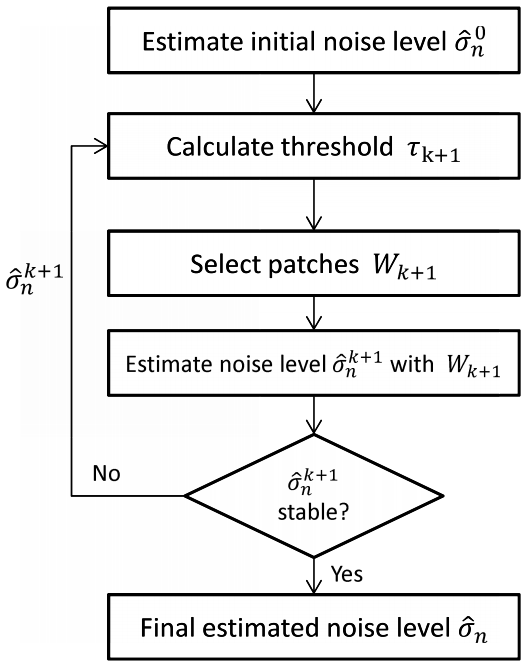
\includegraphics[width=0.9\columnwidth]{single_image_noise_estimation.png}
	\caption{Algorithm for \cite{noise-weak-texture}.}
	\label{fig:alg-weak-texture}
\end{figure}
Noise Level Estimation Using Weak Textured Patches of a Single Noisy Image\cite{noise-weak-texture} uses low rank weak textured patches without high frequency components. Noise level is then estimated from selected patches using principal component analysis(PCA). Figure \ref{fig:alg-weak-texture} shows the overall algorithm for this method.

This method is called with default parameters(\(patch\_size=7, decimation\_factor=0, confidence\_interval=0.99, iterations=3\)) in our tests.
% patchsize (optional): patch size (default: 7)
% decim (optional): decimation factor. If you put large number, the calculation will be accelerated. (default: 0)
% conf (optional): confidence interval to determin the threshold for the weak texture. In this algorithm, this value is usually set the value very close to one. (default: 0.99)
% itr (optional): number of iteration. (default: 3)
\subsection{Filtering Framework}\label{ss:filter-framework}
SD Filter\cite{ham2015robust} utilizes both static and dynamic guidance images to preserve structure of the high detailed image and local features.

Filter will be tested on TRICLOBS\cite{triclobs} database. The database includes several captures of different wavelengths. Six scenarios will be tested:
\begin{itemize}
	\item LWIR as static guidance to NIR
	\item LWIR as static guidance to Visible
	\item NIR as static guidance to LWIR
	\item NIR as static guidance to Visible
	\item Visible as static guidance to LWIR
	\item Visible as static guidance to NIR
\end{itemize}

Source code of the filter is available on the web via github\cite{github:sdfilter}. The code will be used on this project. If playing with parameters is not enough to get good results, the source code will be modified.

\section{Experiments}

To evaluate the performance of the SD Filter\cite{ham2015robust} on TRICLOBS\cite{triclobs} dataset, we are going to use two different sigma estimation methods. Six input-guidance scenarios is going to be tested on TRICLOBS which has  16 different motion sequences representing different military and civilian surveillance scenarios dataset.TRICLOBS dataset features NIR and LWIR outside of visible spectrum. 

\subsection{Sigma Estimation Methods}
As the first part of this project, the sigma estimation methods are tested on a synthetic noisy image. Random noise with different sigma levels are added to the original noise-free image and the methods are evaluated.

For testing 100 noisy images are generated from the same image to simulate a static, noisy scene for Method\ref{ss:online-var}. Method \ref{ss:weak-tex} is called with its default settings; patch size 7, no decimation, 0.99 confidence threshold, and 3 iterations. Noise levels for this experiment are; 2, 5, 10, 20 and 30.

\begin{table}[h!]
	\centering
	\caption{Sigma Estimation Test Results}
	\label{tab:sigma-est}
	\begin{tabular}{cccc}
		\toprule
		\bfseries Sigma Value & \bfseries Method & \bfseries Estimated Value & \bfseries Error Rate\\
		\midrule
		\multirow{2}{*}{\(\sigma=2\)} & Method1 & 1.99 & 0.52 \% \\
		& Method2 & 1.93 & 3.61 \% \\
		\multirow{2}{*}{\(\sigma=5\)} & Method1 & 4.87 & 2.56 \% \\
		& Method2 & 4.75 & 5.04 \% \\
		\multirow{2}{*}{\(\sigma=10\)} & Method1 & 9.59 & 4.07 \% \\
		& Method2 & 9.39 & 6.10 \% \\
		\multirow{2}{*}{\(\sigma=20\)} & Method1 & 18.79 & 6.04 \% \\
		& Method2 & 18.41 & 7.97 \% \\
		\multirow{2}{*}{\(\sigma=30\)} & Method1 & 27.68 & 7.72 \% \\
		& Method2 & 27.18 & 9.41 \% \\
		\bottomrule
	\end{tabular}
\end{table}

\autoref{tab:sigma-est} shows results for this experiment. The results look promising for both methods. Estimated values are below 10 \% error mark until sigma level goes up to 30 and that is a high noise level for an 8bit image.

The real problem with this experiment is that the results might not hold true for actual sensor noise. In that scenario we might have to go with adding a synthetic noise on top of an already noisy image.

\subsection{Filter Performance Evaluation}
In this section filtering frameworks inputs and outputs will be fed to two different noise - or sigma - estimation methods. Estimated values will be used to evaluate the performance this filtering framework for various scenarios mentioned in  \ref{ss:filter-framework} -  \nameref{ss:filter-framework}. These scenarios are executed on 3 different scenes(TRI\_A1, TRI\_A2, TRI\_A4) from TRICLOBS\cite{triclobs} dataset. 

Scenes are selected as static as possible to allow Method\ref{ss:online-var} to work. For each scene at least 10 frames are used as prior tests for sigma estimation revealed more images doesn't mean more precise value estimation.
\begin{table}[!h]
	\centering
	\caption{Filter parameters}
	\label{tab:filter-parameters}
	\begin{tabular}{ccc}
		\hline
		\(\lambda\) & \(\mu\) & \(\nu\) \\ \hline
		3           & 300     & 15      \\
		7           & 600     & 30      \\
		15          & 900     & 45      \\ \hline
	\end{tabular}
\end{table}

Each case is run with 27 different settings.\autoref{tab:filter-parameters} shows a combination of values used for our testing. Best values with lowest post-filter noise levels are given at each section.
Best parameters are used to analyze the characteristics of the filter better.
\subsubsection{LWIR guiding NIR}
In this case LWIR image is used as static guidance to filter noise on NIR image. \autoref{tab:lwir-nir-params} shows parameters used in this experiment.
\begin{table}[!ht]
	\centering
	\caption{Parameters used for LWIR guiding NIR}
	\label{tab:lwir-nir-params}
	\begin{tabular}{@{}cccl@{}}
		\toprule
		\bfseries Sigma Value & \(\lambda\) & \(\mu\) & \(\nu\) \\ \midrule
		TRI\_A1               & 1.99        & 0.52 \% & 123       \\
		TRI\_A2               & 4.87        & 2.56 \% & 123        \\
		TRI\_A4               & 27.68       & 7.72 \% & 123        \\ \bottomrule
	\end{tabular}
\end{table}
\subsubsection{LWIR guiding Day-light}
In this case LWIR image is used as static guidance to filter noise on Day-light image. \autoref{tab:lwir-day-params} shows parameters used in this experiment.
\begin{table}[!ht]
	\centering
	\caption{Parameters used for LWIR guiding Day-light}
	\label{tab:lwir-day-params}
	\begin{tabular}{@{}cccl@{}}
		\toprule
		\bfseries Sigma Value & \(\lambda\) & \(\mu\) & \(\nu\) \\ \midrule
		TRI\_A1               & 1.99        & 0.52 \% & 123       \\
		TRI\_A2               & 4.87        & 2.56 \% & 123        \\
		TRI\_A4               & 27.68       & 7.72 \% & 123        \\ \bottomrule
	\end{tabular}
\end{table}
\subsubsection{NIR guiding LWIR}
In this case NIR image is used as static guidance to filter noise on LWIR image. \autoref{tab:nir-lwir-params} shows parameters used in this experiment.
\begin{table}[!ht]
	\centering
	\caption{Parameters used for NIR guiding LWIR}
	\label{tab:nir-lwir-params}
	\begin{tabular}{@{}cccl@{}}
		\toprule
		\bfseries Sigma Value & \(\lambda\) & \(\mu\) & \(\nu\) \\ \midrule
		TRI\_A1               & 1.99        & 0.52 \% & 123       \\
		TRI\_A2               & 4.87        & 2.56 \% & 123        \\
		TRI\_A4               & 27.68       & 7.72 \% & 123        \\ \bottomrule
	\end{tabular}
\end{table}
\subsubsection{NIR guiding Day-light}
In this case NIR image is used as static guidance to filter noise on Day-light image. \autoref{tab:nir-day-params} shows parameters used in this experiment.
\begin{table}[!ht]
	\centering
	\caption{Parameters used for NIR guiding Day-light}
	\label{tab:nir-day-params}
	\begin{tabular}{@{}cccl@{}}
		\toprule
		\bfseries Sigma Value & \(\lambda\) & \(\mu\) & \(\nu\) \\ \midrule
		TRI\_A1               & 1.99        & 0.52 \% & 123       \\
		TRI\_A2               & 4.87        & 2.56 \% & 123        \\
		TRI\_A4               & 27.68       & 7.72 \% & 123        \\ \bottomrule
	\end{tabular}
\end{table}
\subsubsection{Day-light guiding LWIR}
In this case Day-light image is used as static guidance to filter noise on LWIR image. \autoref{tab:day-lwir-params} shows parameters used in this experiment.
\begin{table}[!ht]
	\centering
	\caption{Parameters used for Day-light guiding LWIR}
	\label{tab:day-lwir-params}
	\begin{tabular}{@{}cccl@{}}
		\toprule
		\bfseries Sigma Value & \(\lambda\) & \(\mu\) & \(\nu\) \\ \midrule
		TRI\_A1               & 1.99        & 0.52 \% & 123       \\
		TRI\_A2               & 4.87        & 2.56 \% & 123        \\
		TRI\_A4               & 27.68       & 7.72 \% & 123        \\ \bottomrule
	\end{tabular}
\end{table}
\subsubsection{Day-light guiding NIR}
In this case Day-light image is used as static guidance to filter noise on NIR image. \autoref{tab:day-nir-params} shows parameters used in this experiment.
\begin{table}[!ht]
	\centering
	\caption{Parameters used for Day-light guiding NIR}
	\label{tab:day-nir-params}
	\begin{tabular}{@{}cccl@{}}
		\toprule
		\bfseries Sigma Value & \(\lambda\) & \(\mu\) & \(\nu\) \\ \midrule
		TRI\_A1               & 1.99        & 0.52 \% & 123       \\
		TRI\_A2               & 4.87        & 2.56 \% & 123        \\
		TRI\_A4               & 27.68       & 7.72 \% & 123        \\ \bottomrule
	\end{tabular}
\end{table}
{\small
\bibliographystyle{ieee}
\bibliography{egbib}
}

\end{document}
